% This is the master file of the folder structure.

% First, the preamble needs to be called. This contains all the 'under the hood' stuff for your document.
% Use \input rather than than \include for .tex files, because \input can be nested and don't include a page break.
% This file contains your LaTeX preamble. A preamble is a part of your document where all required packages and macros can be defined. This needs to be done before the \begin{document} command.

% Documentclass:
% Standard LaTeX classes are: article, book, report, slides, and letter. These cover the basis, but are not best. More advanced users might want to try out the KOMA classes or the memoir class. Optional arguments: 10pt. The font size of the main content is set to 10pt with the option between [].
\documentclass{llncs}
\usepackage[utf8]{inputenc}

% Geometry:
% The papersize of the document is defined with the geometry package. Here, the size is set to A4 with a4paper. Other possibilities are a5paper, b5paper, letterpaper, legalpaper and executivepaper.
\usepackage[a4paper]{geometry}

% AMS math packages:
% Required for proper math display.
%\usepackage{amsmath,amsfonts,amsthm}	% conflict with the llncs package
\usepackage{amsmath,amsfonts}			% to avoid conflict with the llncs package
%\usepackage{amsfont} create a conflict so it's not used
\usepackage{amssymb}
\usepackage{mathtools}
% For case equation with nested label
% \usepackage{cases} NOT USEFUL



% Graphicx:
% If you want to include graphics in your document, the graphicx package is required.
\usepackage{graphicx}

% Graphic path declaration:
\graphicspath{{figs/}}

% Tabu:
% To test if this package could be the latest package for my work
\usepackage{tabu}

% [OLD] Booktabs:
% The booktabs package is needed for better looking tables. 
\usepackage{booktabs}

% [OLD] Tables:
\usepackage[table]{xcolor}
\usepackage{multirow}
%\usepackage{tabularx}

\newcommand{\win}{\cellcolor[gray]{0.9}}

% Enumeration:
% To manipulate the listing of object
\usepackage[inline]{enumitem}
\setlist*[enumerate,1]{%
	label=(\roman*),
}
% [Alternative]
%\usepackage{easylist}

% SIunitx:
% The SIunitx package enables the \SI{}{} command. It provides an easy way of working with (SI) units.
\usepackage{siunitx}

% URL:
% Clickable URL's can be made with this package: \url{}.
%\usepackage{url}

% Caption:
% For better looking captions. See caption documentation on how to change the format of the captions.
%\usepackage{caption}

% Hyperref:
% This package makes all references within your document clickable. By default, these references will become boxed and colored. This is turned back to normal with the \hypersetup command below.
\usepackage{hyperref}
\hypersetup{colorlinks=false,pdfborder=0 0 0}

% Cleveref:
% This package automatically detects the type of reference (equation, table, etc.) when the \cref{} command is used. It then adds a word in front of the reference, i.e. Fig. in front of a reference to a figure. With the \crefname{}{}{} command, these words may be changed.
\usepackage{cleveref}
\crefname{equation}{equation}{equations}
\crefname{figure}{figure}{figures}	
\crefname{table}{table}{tables}

% Pseudo code packages:
\usepackage[ruled,linesnumbered]{algorithm2e}
\usepackage{algorithmicx}
\usepackage{algpseudocode}

% Verbatim:
% Typewriter formatting and comment environment
\usepackage{verbatim}

% Bibliography style
%\usepackage{natbib}



% Command

% For the level structure depending of the 

% The title page is created with the command \maketitle which needs to be placed after the \begin{document} command. To create the titlepage, some entries are needed: the name of the autor is defined by \author{}, the title by the entry \title{} and the date by the command \date{}. Note that the current date is displayed with \today.
\author{Luca Ambrosini \and Giancarlo Nicol\`{o}}
\title{ALC}
\date{}

%\titlerunning{<Your abbreviated contribution title>}
%\authorrunning{<abbreviated author list>}
\institute{Univesitat Polit\`{e}cnica De Val\`{e}ncia}
%	\and <name of the next institute>}

% All the actual content of your document should be placed after \begin{document} and before \end{document}. This content should be placed in the docs folder and can then be called with \input{docs/filename}.
\begin{document}

% Here the actual title page is printed, based on the given entries \author{}, \title{} and \date{}.
\maketitle

% The table of contents can be automatically generated with the \tableofcontents command. Note that you need to compile the document twice in order to see the changes in the table of contents.
%\tableofcontents

% List of figures
%\listoffigures
 
% List of tables
%\listoftables

% The list of algorithm
%\listofalgorithms

% The \input{} command reads and processes the indicated example.tex file. Note that docs/ locates the folder where the .tex file is stored.
\abstract

Version one

This paper describes an explorative approach to create from scratch a set of baselines for tackling tweet classification problems using natural language processing and machine learning techniques.
Our approach focuses on neural network models taken from state of the art that exploit different corpus preprocessing, tweets representations and features extraction methods.
Finally, we will discuss how we applied this methodology to the \emph{Classification Of Spanish Election Tweets (COSET)} task at IberEval 2017 and present the results we obtained

Version two

This paper describes our participation in the \emph{Classification Of Spanish Election Tweets (COSET)} task at IberEval 2017.
During the searching process for the best classification system to send for the competition, we developed a comparative study over possible combination of corpus preprocessing, text representations and classification models. After an initial models exploration, we focus our attention over specific neural models.
Interesting insight can be drawn from the comparative study helping future practitioner tackling tweets classification problems to create system baseline for their work.

Possible add for the report in general and 

handcrafted features

explain that we haven't put a proper module for handcrafted features, but our modular approach to solve the classification problem lead to an easy customization and integration of a proper module for these handcrafted features.		% Abstract
\section{Introduction} \label{sec:introduction}

Intro over nlp and text classification: motivation why this field is important and the actual challenge and open problems (will be top just to list some problem and their way to be solved, for example citing the different workshop that we had during the course)


Text classification is an important task in Natural Language Processing with many applications, such as web search, information retrieval, ranking and document classification (Deerwester et al., 1990; Pang and Lee, 2008). Recently, models based on neural networks have become increasingly popular (Kim, 2014; Zhang and LeCun, 2015; Conneau et al., 2016). While these models achieve very good performance in practice, they tend to be relatively slow both at train and test time, limiting their use on very large datasets.

The 

vedi citazioni su word embedding di mark e bag of word da maite

Introduce informally our task and list some way of tackling this problem from the different perspectives, maybe say that we de-construct tthe actual approach and cathegorized their inner process in: representation, preprocessing, model and post processing (that we haven't done).

Finally explain how we structured this report

In the following we firstly describe the 

In this paper we describe our participation for addressing
the PR-SOCO task. The rest of the paper is organized as
follows. Next section is devoted to dene the Personality
Recognition task. In Section 4 the model proposed is described.
Following, in Section 5, the results achieved are
presented. Finally, in Section 6 our results are discussed,
and future work is proposed.


	% Introduction
\section{Task definition} \label{sec:task}

The COSET shared task's aim was to classify Spanish written tweets talking about the 2015 Spanish General Election, where each tweet had to be classified into one of five different categories:
\begin{enumerate*}
\item political issues, related to the most abstract electoral confrontation; 
\item policy issues, about sectorial policies; 
\item personal issues, on the life and activities of the candidates; 
\item campaign issues, related with the evolution of the campaign;
\item and other issues.
\end{enumerate*}

Participants had access to a labelled corpus composed of training set (2242 tweets) and development set (250 tweets) for system benchmarking. We analysed it and find the following statistical information that guided us in the baselines building:
\begin{multicols}{2}
\begin{itemize}
	\item Average train sequence length:
	\begin{itemize}
		\item 135 chars 
		\item 24 words
	\end{itemize}
	\item Max train sequence length: 
	\begin{itemize}
		\item 140 chars
		\item 49 words
	\end{itemize}
\end{itemize}
\end{multicols}			% Task description
\section{Systems description} \label{sec:methods}

\textbf{giancarlo modifications: I've changed a little bit the structure to create a kind of flux over the contents. The main idea is to switch the mind set from METHOD $\rightarrow$ (CLASSIFICATION) SYSTEM, in this way we can report our work from a software engineer point of view, analysing each part/process as a module. It seams stupid, but in this way I have a name fro each step of the METHOD/SYSTEM and I suppose can help the readers to better understand what we have done.}


In this section we are going to describe the tweets classification systems built, from a module perspective we can describe our systems as composed of three main blocks: text pre-preprocessor (\cref{subsec:preprocessing}),  text representation (\cref{subsec:representation}) and classification model (\cref{subsec:classificationModel}). 


\subsection{Initial investigation} \label{subsec:boh}
To address the tweets classification problem we began our investigation analysing some of the most widely used text representations and classifiers.
We began analysing possible text representations focusing our attention on lexical features based: \emph{Bag Of Words} \cite{harris1954distributional},\emph{Bag Of N-Grams} (bigrams and trigrams), both with and without \emph{term frequency-inverse document frequency} normalization (i.e. TF-IDF norm).
Regarding possible classifiers exploiting above representations,  we analysed \emph{Random Forest, Decision Trees, Support Vector Machines} and \emph{Multi Layer Perceptron}, but since the results obtained with the combination of those \emph{model + representation} were outperformed by neural network based models, we decided not to report their analysis in this paper, but rather focus the modules description in relation to neural models.


\subsection{Text preprocessing} \label{subsec:preprocessing}


We explored different combinations of twitter pre-processing, as converting some elements such mentions, emoji, smiley, hashtags into constant string (i.e. Tokenize @Ambros and \#atoppe :) $\rightarrow $ Tokenize \$MENTION and \$HASHTAG \$SMILEY ); removeing elements as URLs, reserved words and numbers.
We also measured the contribution of stemming, stopwords and punctuation removal.
To address those pre-processing we used the following \cite{nltk} \cite{tweets-preprocessor}.

\subsection{Text representation} \label{subsec:representation}
As a tweet representation used as first layer

To represent to tweet fed into the classifier we decided to used word embeddings,which is a tecnique where elements (in our case words and n-grams) are mapped into a vector of real numbers.
The whole sentence is mapped into a matrix with dimension \emph{sentence lenght} $\times$ \emph{embedding dimension}.
We left the sentence length as a parameter and the best results were obtained with length=30, that's reasonable since the average tweet length in words in 24.
If the sentence dimension is bigger than the selected window we used the first length words, if the sentence is smaller than the windwos we used 0-right padding.

\subsubsection{Words vectors}
Since the number of tweets is considered small to learn vector representation of words, we tried to initialize the embedding matrix with pretrained word vectors.
In particular we used vectors trained on wikipedia using fastText \cite{bojanowski2016enriching}.
We tried static pretrained vectors, learning them during training starting from a random matrix or from the pretrained embeddings.

\subsubsection{N-gram embedding}
We also tried to learn an embedding for n-grams (bigrams and trigrams), but, since the corpus is small, n-grams frequencies are very low and the algorithm is not able to learn a valid embedding.
Also there are no pre-trained n-grams embeddings available.
Bigrams brought a small improvement, bigger n-grams result in performance decrease.



\subsection{Classification models} \label{subsec:classificationModel}
In the following section we present different neural network models, each model has as first layer an embedding layer that maps words to the corresponding word vectors, as described in the previous section.


\subsubsection{Convolutional Neural Network}
Convolutional Neural Networks are considered state of the art in many text classification problem. (GIANCARLO, citazioni?)
This model is composed by a convolutional layer, followed by a global max pooling layer and two fully connected layers.

\subsubsection{Long short-term memory}
LSTM is a type of Recurrent Neural Network that is relatively insensitive to gap length, compared to others RNN, they are considered state of the art in many NLP topics, like machine translation.
In this model the classical embedding layer is followed by an LSTM layer with 128 units, terminated by a fully connected layer.
We also tried Bidirectional LSTM, since they are bringing an improvement in different tasks, but they are performing worst on our use case.

\subsubsection{Fast text}
This model is based on this paper \cite{joulin2016bag}.
Differently to the other models where just words are used, here Bag of n-grams are added to the input as  additional features to capture some partial information about the local word order.
It this model the embedding output is directly fed into a \emph{GlobalAveragePooling} layer, that transofrms the whole sentece in a single vector computed as the average of the word vectors.
This vector is then projected into 2 fully connected layers. In the paper the number of hidden layers is fixed to 10, but we measured better performance using just 2 layers.
\begin{figure}[h]
\centering
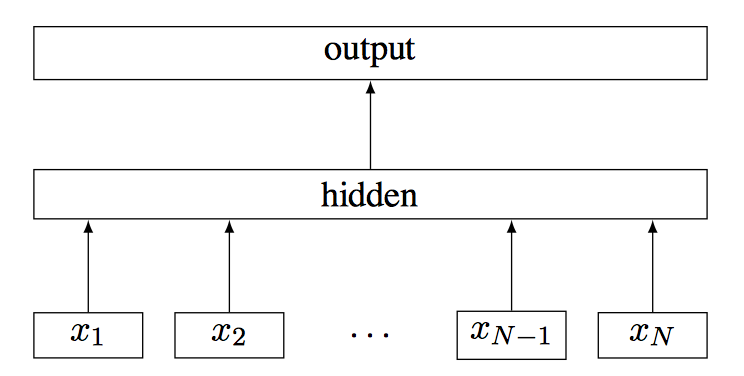
\includegraphics[width=.75\columnwidth]{fast_text}
\caption{\cite{joulin2016bag} Model architecture of \emph{fastText} for a sentence with $N$ n-gram features $x_1,\dots,x_N$. The features are embedded and averaged to form the hidden variable.}
\label{fig:fastText}
\end{figure}
\textbf{@ Luca: Source:  }


\subsubsection{KIM.}

\textbf{@ Luca: Source: Zhang, Y., \& Wallace, B. (2015). A Sensitivity Analysis of (and Practitioners’ Guide to) Convolutional Neural Networks for Sentence Classification.}
\textbf{http://www.wildml.com/2015/11/understanding-convolutional-neural-networks-for-nlp/}

\begin{figure}[h]
\centering
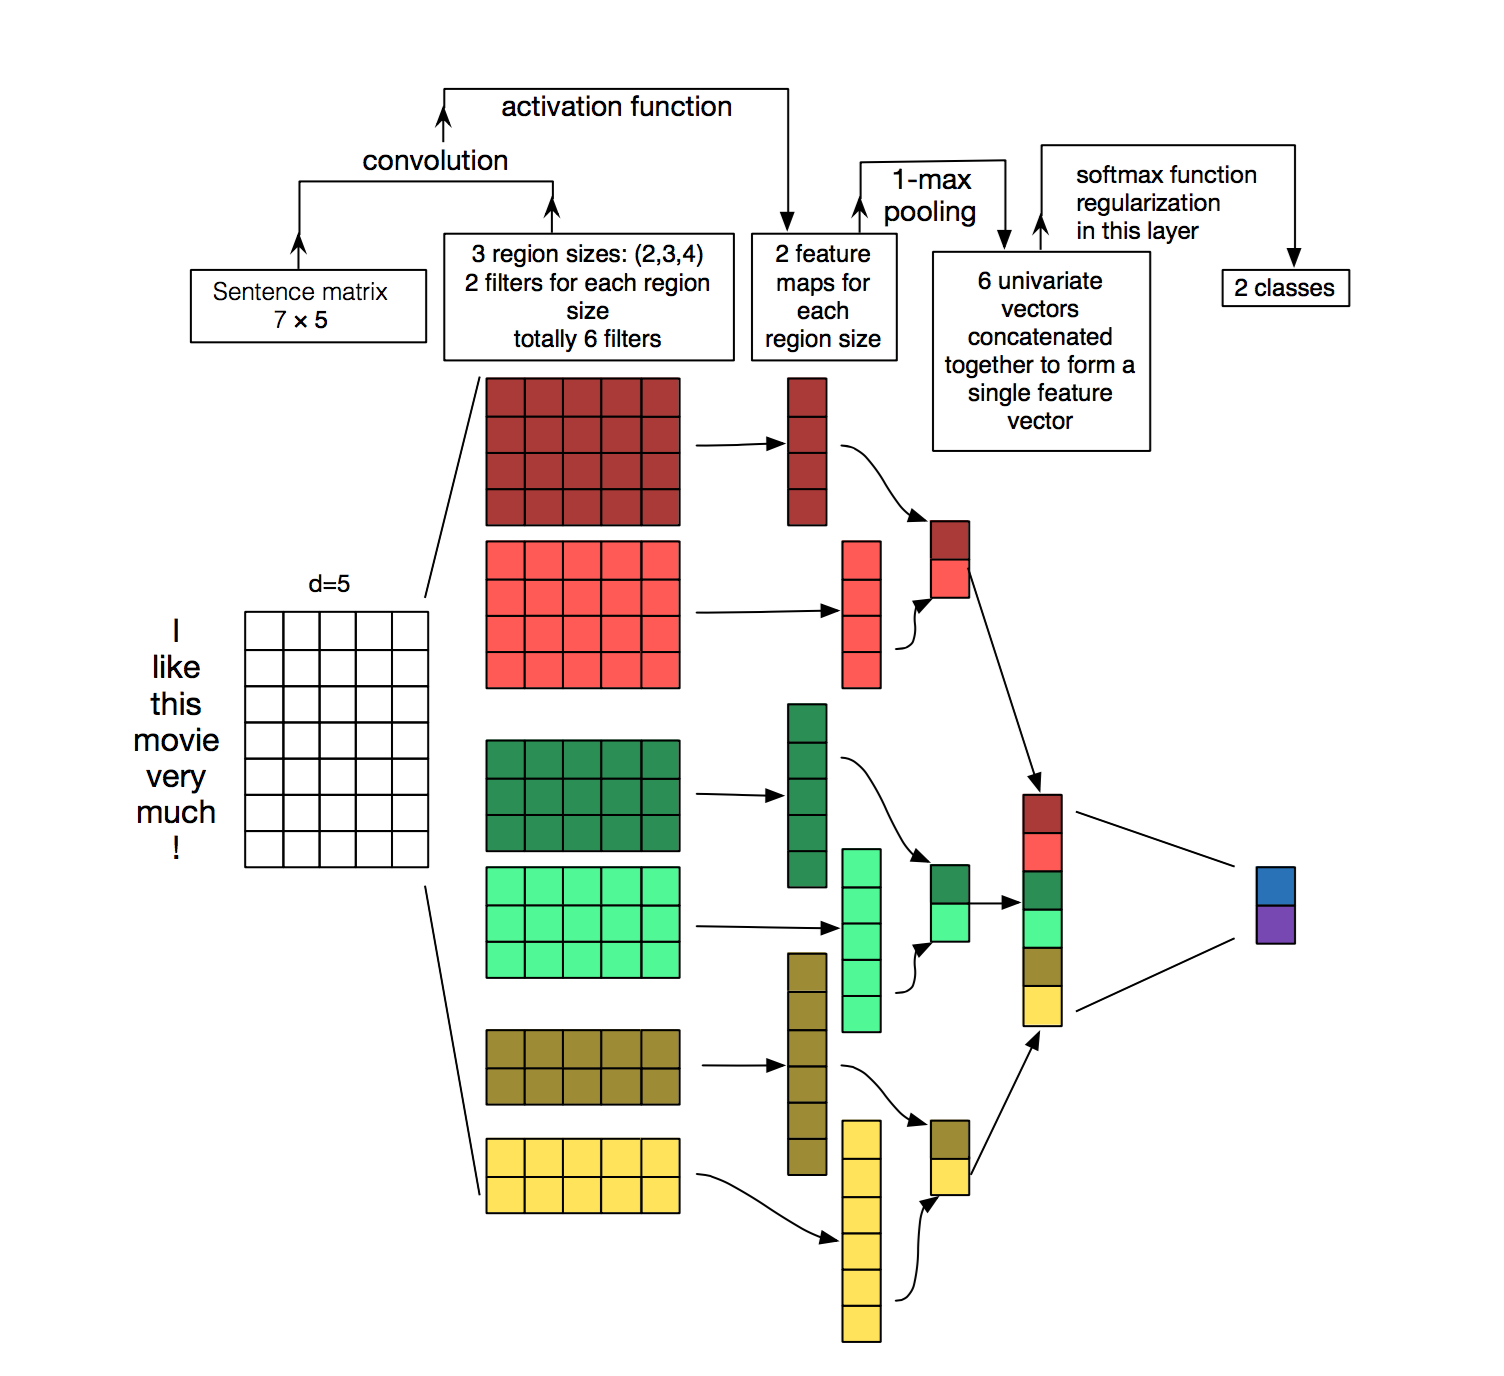
\includegraphics[width=.75\columnwidth]{kim_cnn}
\caption{Illustration of a Convolutional Neural Network (CNN) architecture for sentence classification}
\label{fig:kim}
\end{figure}
\textbf{@giancarlo: Non penso che ants\_example vada esattamente qui :D}


This model is based on this paper \cite{kim2014convolutional}. It is based on different filter region size convolutions, followed by maxpooling layers.
All those outputs are concatenated to build sentence representation that is finally projected into a dense layer for the classification.
The intuition behind this model is that smaller filter region size should be able to capture short sentence patterns (similar to ngrams), while bigger sizes should capture sentence level features. We reached the best performance using [2, 3, 5, 7] as filter sizes.
		% Systems description
\section{Evaluation} \label{sec:evaluation}

\subsection{Metrics}

\begin{equation}
F_{1-macro} = \frac{1}{|L|} \displaystyle\sum_{l\in L} F_1(y_l, \hat{y}_l)
\end{equation}

\begin{equation}
F_1 = 2 \cdot \frac{precision \cdot recall }{precision + recall}
\end{equation}

\begin{equation}
precision = \frac{1}{|L|} \displaystyle\sum_{l\in L} Pr(y_l, \hat{y}_l)
\end{equation}

\begin{equation}
recall = \frac{1}{|L|} \displaystyle\sum_{l\in L} R(y_l, \hat{y}_l)
\end{equation}


\subsection{Results}

Put an intro over the results that will be analyzed and then comments over them

table of only the 5 models main models and 6 kind of preprocessing
only the mean and say that is 10 fold CV

table of word representation




		% Systems evaluations
\section{Conclusions} \label{sec:conclusion}

In this paper we have presented our participation in the IberEval2017 Classification Of Spanish Election Tweets (COSET) shared task. Five different neural models were explored, in combination with 11 types of preprocessing. No preprocessing emerged to be the best with every kind of model, indicating that the preprocessing pipeline optimization has a big impact on results.
We also explored static vs non-static word embeddings and non-static vectors initialized with pre-trained vectors on a bigger corpus is the best performing combination.


	% Conclusions



% The bibliography is printed with \bibliography{}. With the command \bibliographystyle{} a style is picked.
%\bibliographystyle{plain} 		% for [1] cite style
%\bibliographystyle{plainnat}	% for [Surname et al] cite style
\bibliographystyle{splncs}		% FOR LNCS
%\bibliography{refs/references}
\begin{thebibliography}{1}

\bibitem{kim2014convolutional}
Kim, Yoon. "Convolutional neural networks for sentence classification." arXiv preprint arXiv:1408.5882 (2014).

\bibitem{joulin2016bag}
Joulin, Armand, et al. "Bag of tricks for efficient text classification." arXiv preprint arXiv:1607.01759 (2016).

\bibitem{nltk}
Edward Loper and Steven Bird. 2002. NLTK: the Natural Language Toolkit. In Proceedings of the ACL-02 Workshop on Effective tools and methodologies for teaching natural language processing and computational linguistics - Volume 1 (ETMTNLP '02), Vol. 1. Association for Computational Linguistics, Stroudsburg, PA, USA, 63-70. DOI=http://dx.doi.org/10.3115/1118108.1118117

\bibitem{tweets-preprocessor}
Preprocessor is a preprocessing library for tweet data written in Python, https://github.com/s/preprocessor
\end{thebibliography}	% Conclusions

% To close your document, add the \end{document} command. Everything after this command will not be processed.
\end{document}